\documentclass[xcolor=pdftex,dvipsnames,table,mathserif,aspectratio=169]{beamer}
\usetheme{default}
\usetheme{metropolis}
\usepackage{minted}
\usepackage{mathtools}
\setbeamersize{text margin left=.3in,text margin right=.3in} 

\usepackage[english]{babel}
\usepackage{pgf,pgfarrows,pgfnodes,pgfautomata,pgfheaps}
\usepackage{amsmath,amssymb,setspace,centernot}
\usepackage[latin1]{inputenc}
\usepackage{pgf,tikz}
\usepackage[T1]{fontenc}
\usepackage{relsize}
\usepackage{pdfpages}
\usepackage[absolute,overlay]{textpos} 


\DeclareMathOperator*{\argmax}{arg\,max}
\DeclareMathOperator*{\argmin}{arg\,min}

\newcommand{\X}{\mathtt{X}}
\newcommand{\Y}{\mathtt{Y}}

%\newcommand{\R}{\mathbb{R}}
%\newcommand{\E}{\mathbb{E}}
%\newcommand{\V}{\mathbb{V}}
\newcommand{\p}{\mathbb{P}}
\newcommand*\df{\mathop{}\!\mathrm{d}}
\newcommand{\del}{\partial}


% imports
\usepackage{xargs}
\usepackage{xpatch}
\usepackage{etoolbox}
\usepackage{pdflscape}
\usepackage{booktabs}
\usepackage{threeparttable}
\usepackage[skip=0.2\baselineskip]{caption}

% command for inputting raw latex
\makeatletter
\newcommand\primitiveinput[1]{\@@input #1 }
\makeatother

% common table command
\newcommandx{\tablecontent}[4]{
    \begin{threeparttable}[!ht]
        \centering
        \caption{#3}
        \vspace{-1em}
        \footnotesize
        \begin{tabular}{#1}
            \primitiveinput{../tables/#2.tex}
        \end{tabular}
        \vspace{-0.2em}
        \begin{tablenotes}[flushleft]
            #4
        \end{tablenotes}
    \end{threeparttable}
}




% \usepackage{slashbox}
\title{Advanced Panel Data: Dynamic Panel}
\author{Chris Conlon }
\institute{NYU Stern }


\newcommand{\norm}[1]{\left\lVert#1\right\rVert}
\newcommand{\R}{\mathbb{R}}
\newcommand{\E}{\mathbb{E}}
\newcommand{\V}{\mathbb{V}}
\newcommand{\ol}{\overline}
%\newcommand{\ul}{\underline}
\newcommand{\pp}{{\prime \prime}}
\newcommand{\ppp}{{\prime \prime \prime}}
\newcommand{\policy}{\gamma}


\newcommand{\fp}{\frame[plain]}

\date{\today}

\begin{document}
\maketitle




\section*{Dynamic Panel Data}

\begin{frame}{Dynamic Panel}
\begin{itemize}
\item Suppose that we also want to include a lagged $y_{i,t-1}$
\begin{eqnarray*}
y_{it} = \rho y_{i,t-1} + x_{it}'\beta + \eta_i + \varepsilon_{it}
\end{eqnarray*}
\item We can treat $\eta_i$ as a \alert{random effect} or a \alert{fixed effect}.
\end{itemize}
\end{frame}

\begin{frame}{Dynamic Panel: Nickell (1981) Bias}
Consider the within transform
\begin{eqnarray*}
(y_{it}-\overline{y}_i) = \rho (y_{i,t-1}-\overline{y}_i) + (x_{it}-\overline{x}_i)'\beta +( \varepsilon_{it}- \overline{\varepsilon}_{i})
\end{eqnarray*}
\begin{itemize}
\item This eliminates the fixed effect.
\item But $Cov(y_{i,t-1}-\overline{y}_i, \varepsilon_{it}- \overline{\varepsilon}_{i}) \neq0$. Why?
\begin{itemize}
\item Both contain past and future values
\item There is a direct relationship between $y$ and $\varepsilon$
\item Bias does not disappear as $N \rightarrow \infty$ (it does as $T\rightarrow \infty$).
\item For small $T$, dynamic panel model is \alert{inconsistent}.
\end{itemize}
\end{itemize}
\end{frame}

\begin{frame}{Dynamic Panel: Bias Alternative}
\begin{eqnarray*}
y_{it} = \rho y_{i,t-1} + x_{it}'\beta + \eta_i + \varepsilon_{it}
\end{eqnarray*}
\begin{itemize}
\item We require the following assumption (\alert{strict exogeneity}):
\begin{eqnarray*}
E\left(\varepsilon_{i t} | x_{i 1}, \ldots, x_{i T}, \eta_{i}\right)=0, \quad t=1, \ldots, T
\end{eqnarray*}
\item But what about $y_{it-1}$? 
\begin{itemize}
\item It is correlated with $\varepsilon_{i,t-1}$ and $\eta_i$ (by construction).
\item With serial correlation it is correlated with $\varepsilon_{it}$
\item This is the usual \alert{endogeneity} concern.
\end{itemize}
\end{itemize}
\end{frame}



\begin{frame}{Dynamic Panel: Differenced Model (Anderson-Hsiao)}
How do we deal with endogeneity? With \alert{instruments}!
\begin{eqnarray*}
y_{it} = \rho y_{i,t-1} + x_{it}'\beta + \eta_i + \varepsilon_{it}
\end{eqnarray*}
Consider the first differences ($s$ is a dummy time index):
\begin{eqnarray*}
E\left[x_{i s}\left(\Delta y_{i t}-\rho \Delta y_{i(t-1)}-\Delta x_{i t}^{\prime} \beta\right)\right]=0
\end{eqnarray*}
Idea:
\begin{itemize}
\item Under \alert{strict exogeneity} of $x_{it}$ we can use both \alert{lags} and \alert{leads} as instruments for $y_{i,t-1}$
\item \alert{Excluded Instruments} $x_{i,s}$ do not have a direct effect on $\Delta y_{i,t-1}$.
\item These moments work even in presence of \alert{serially correlated errors}.
\end{itemize}
\end{frame}


\begin{frame}{Minimal Example: Anderson-Hsiao}
Imagine we have only $T=3$ periods:
\begin{align*}
y_{3}-y_{2}=\alpha\left(y_{2}-y_{1}\right)+\beta_{0}\left(x_{3}-x_{2}\right)+\beta_{1}\left(x_{2}-x_{1}\right)+\left(\varepsilon_{3}-\varepsilon_{2}\right)
\end{align*}
\begin{itemize}
\item $E\left(x_{i s} \Delta \varepsilon_{i 3}\right)=0$ has three instruments $(x_{i1},x_{i2},x_{i3})$.
\item The model is \alert{just identified} with 3 parameters $(\alpha,\beta_0,\beta_1)$.
\item The challenge with this approach is often that it suffers from \alert{weak instruments}.
\begin{itemize}
\item We need a lot of variation in $x_{is}$ across $t$ to make this work.
\item A constant trend isn't going to help either.
\end{itemize}
\end{itemize}
\end{frame}

\begin{frame}{Becker, Grossman, Murphy (1994)}
Study annual cigarette consumption with state-level data:
\begin{align*}
c_{it} = \theta c_{i,t-1} +\beta \theta c_{i,t+1} + \gamma p_{it} + \eta_{i} + \delta_t + v_{it}
\end{align*}
A model of (forward looking) \alert{rational addiction}:
\begin{itemize}
\item $c_{it} = $ Annual per capita cigarette consumption in packs by state.
\item $p_{it} =$ Average cigarette price per pack.
\item $\theta = $ Measure of the extent of addiction (for $\theta > 0$).
\item $\beta= $ Discount factor.
\item Derived from forward looking model of \alert{habit formation} FOC's.
\end{itemize}
\end{frame}


\begin{frame}{Becker, Grossman, Murphy (1994)}
\begin{align*}
c_{it} = \theta c_{i,t-1} +\beta \theta c_{i,t+1} + \gamma p_{it} + \eta_{i} + \delta_t + v_{it}
\end{align*}
\begin{itemize}
\item Marginal utility of wealth can show up in $\gamma$ or $\eta_i$.
\item The errors $v_{it}$ are unobserved life-cycle utility shifters, can be autocorrelated. 
\item Absent addiction $\theta=0$ and serial correlation in prices, we would expect to find dependence over time in $c_{it}$.
\item Conditional on $c_{i,t}| (c_{i,t-1},c_{i,t+1})$ does not depend on $p_{i,t+1}$ or $p_{i,t+1}$.
\end{itemize}
\end{frame}


\begin{frame}{Becker, Grossman, Murphy (1994)}
\begin{align*}
c_{it} = \theta c_{i,t-1} +\beta \theta c_{i,t+1} + \gamma p_{it} + \eta_{i} + \delta_t + v_{it}
\end{align*}
\begin{itemize}
\item Identify $(\theta,\beta,\gamma)$ from the assumption that prices are strictly exogenous
\item Use lagged and future $p_{i,t+s}$ and $p_{i,t-s}$ as IV. 
\item Use the change in cigarette taxes.
\item Consumers need to fully anticipate \alert{future price changes} for this to work.
\end{itemize}
\end{frame}

\begin{frame}{Becker, Grossman, Murphy (1994): Table 1}
\begin{center}
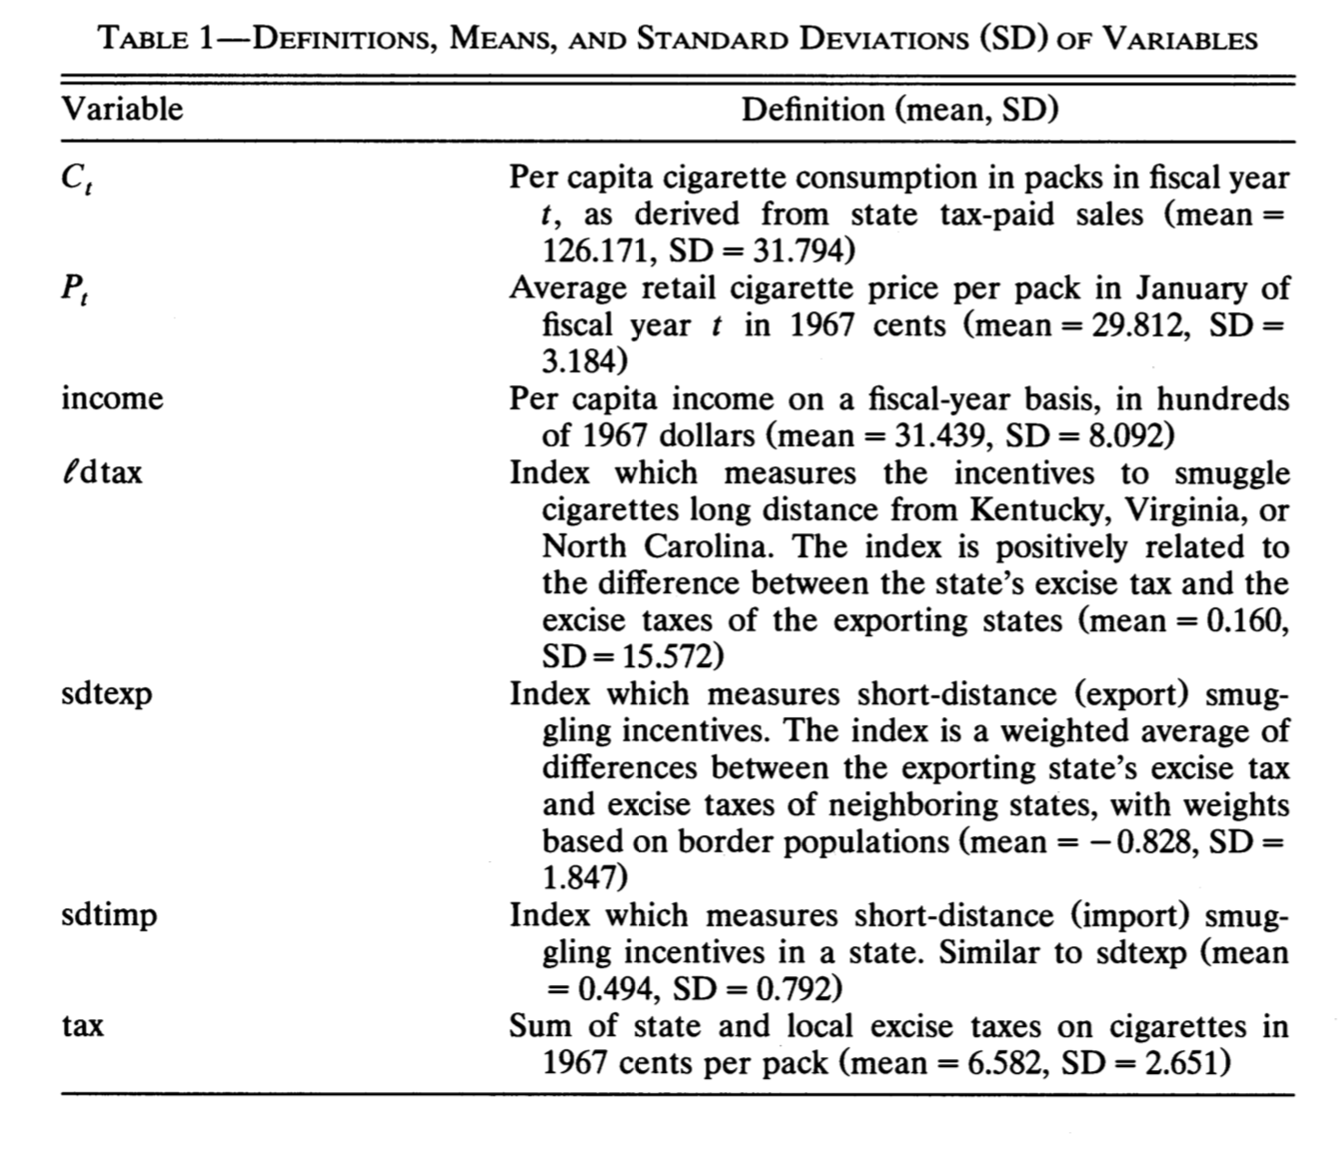
\includegraphics[width=3in]{./resources/gbm_t1.png}
\end{center}
\end{frame}

\begin{frame}{Becker, Grossman, Murphy (1994): Table 2}
\begin{center}
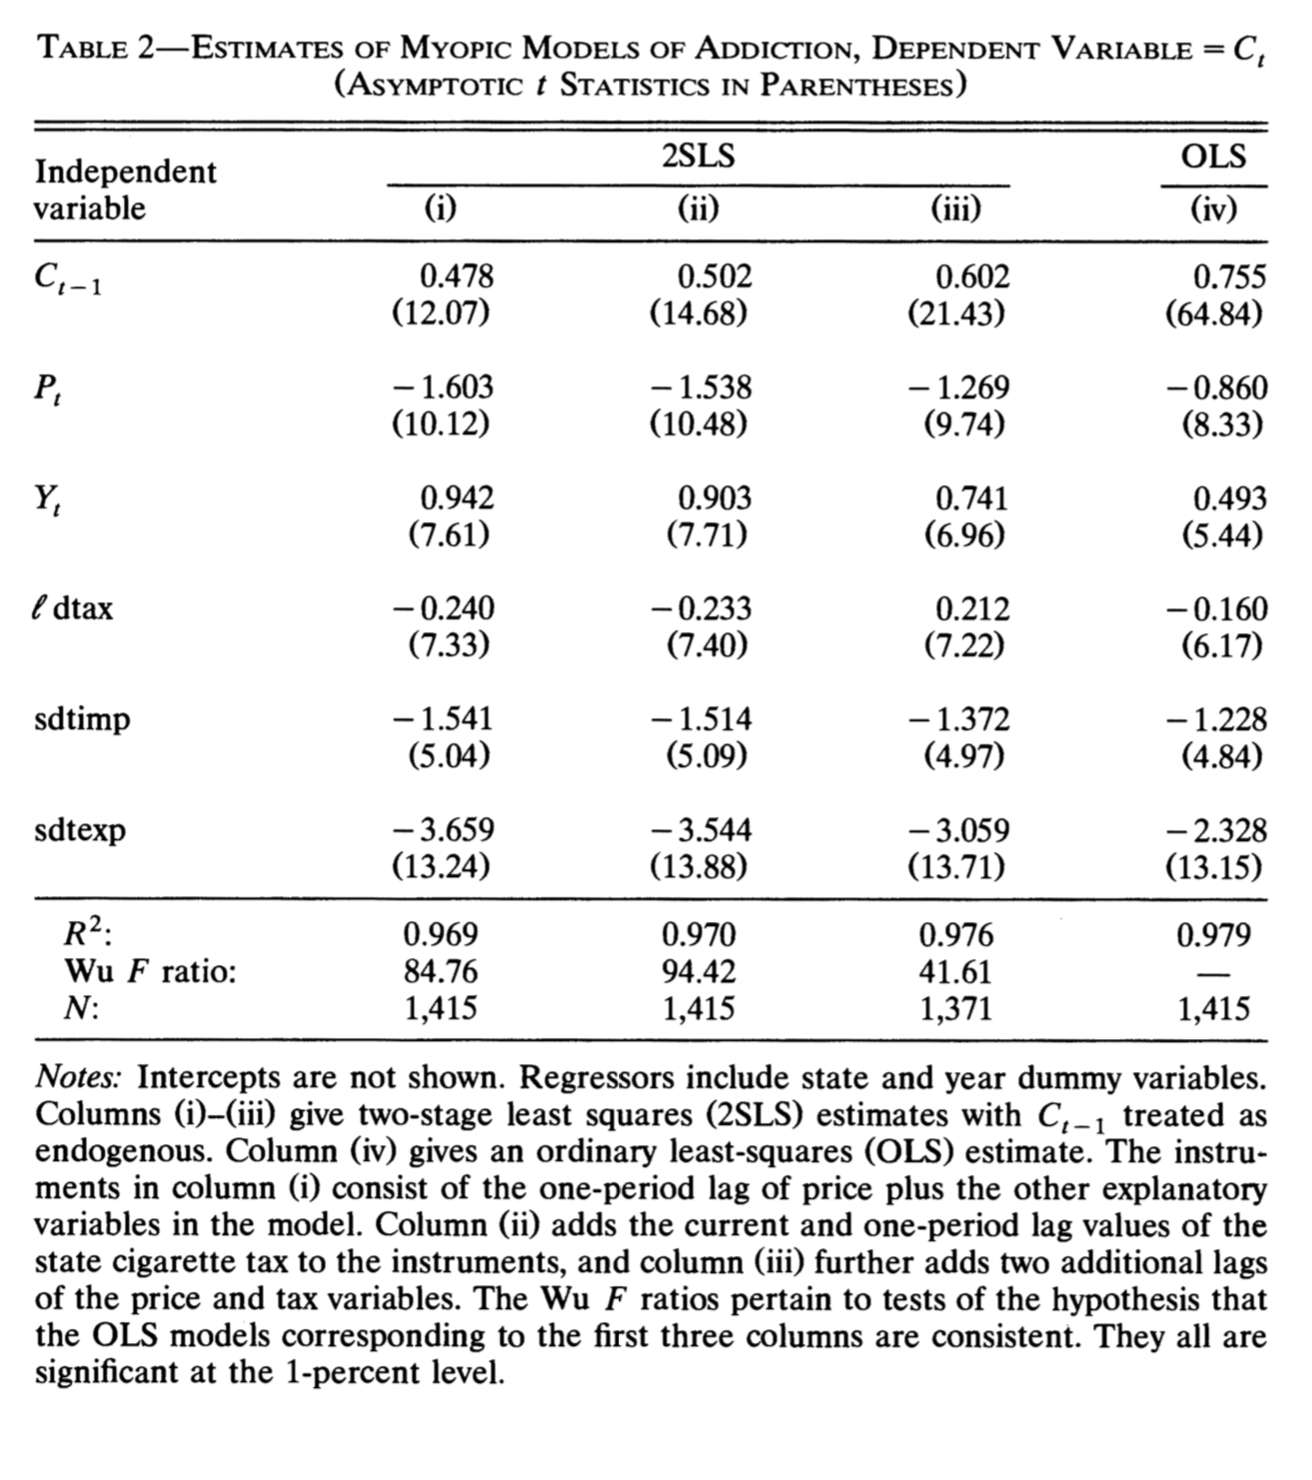
\includegraphics[width=2.8in]{./resources/gbm_t2.png}
\end{center}
\end{frame}

\begin{frame}{Becker, Grossman, Murphy (1994): Table 3}
\begin{center}
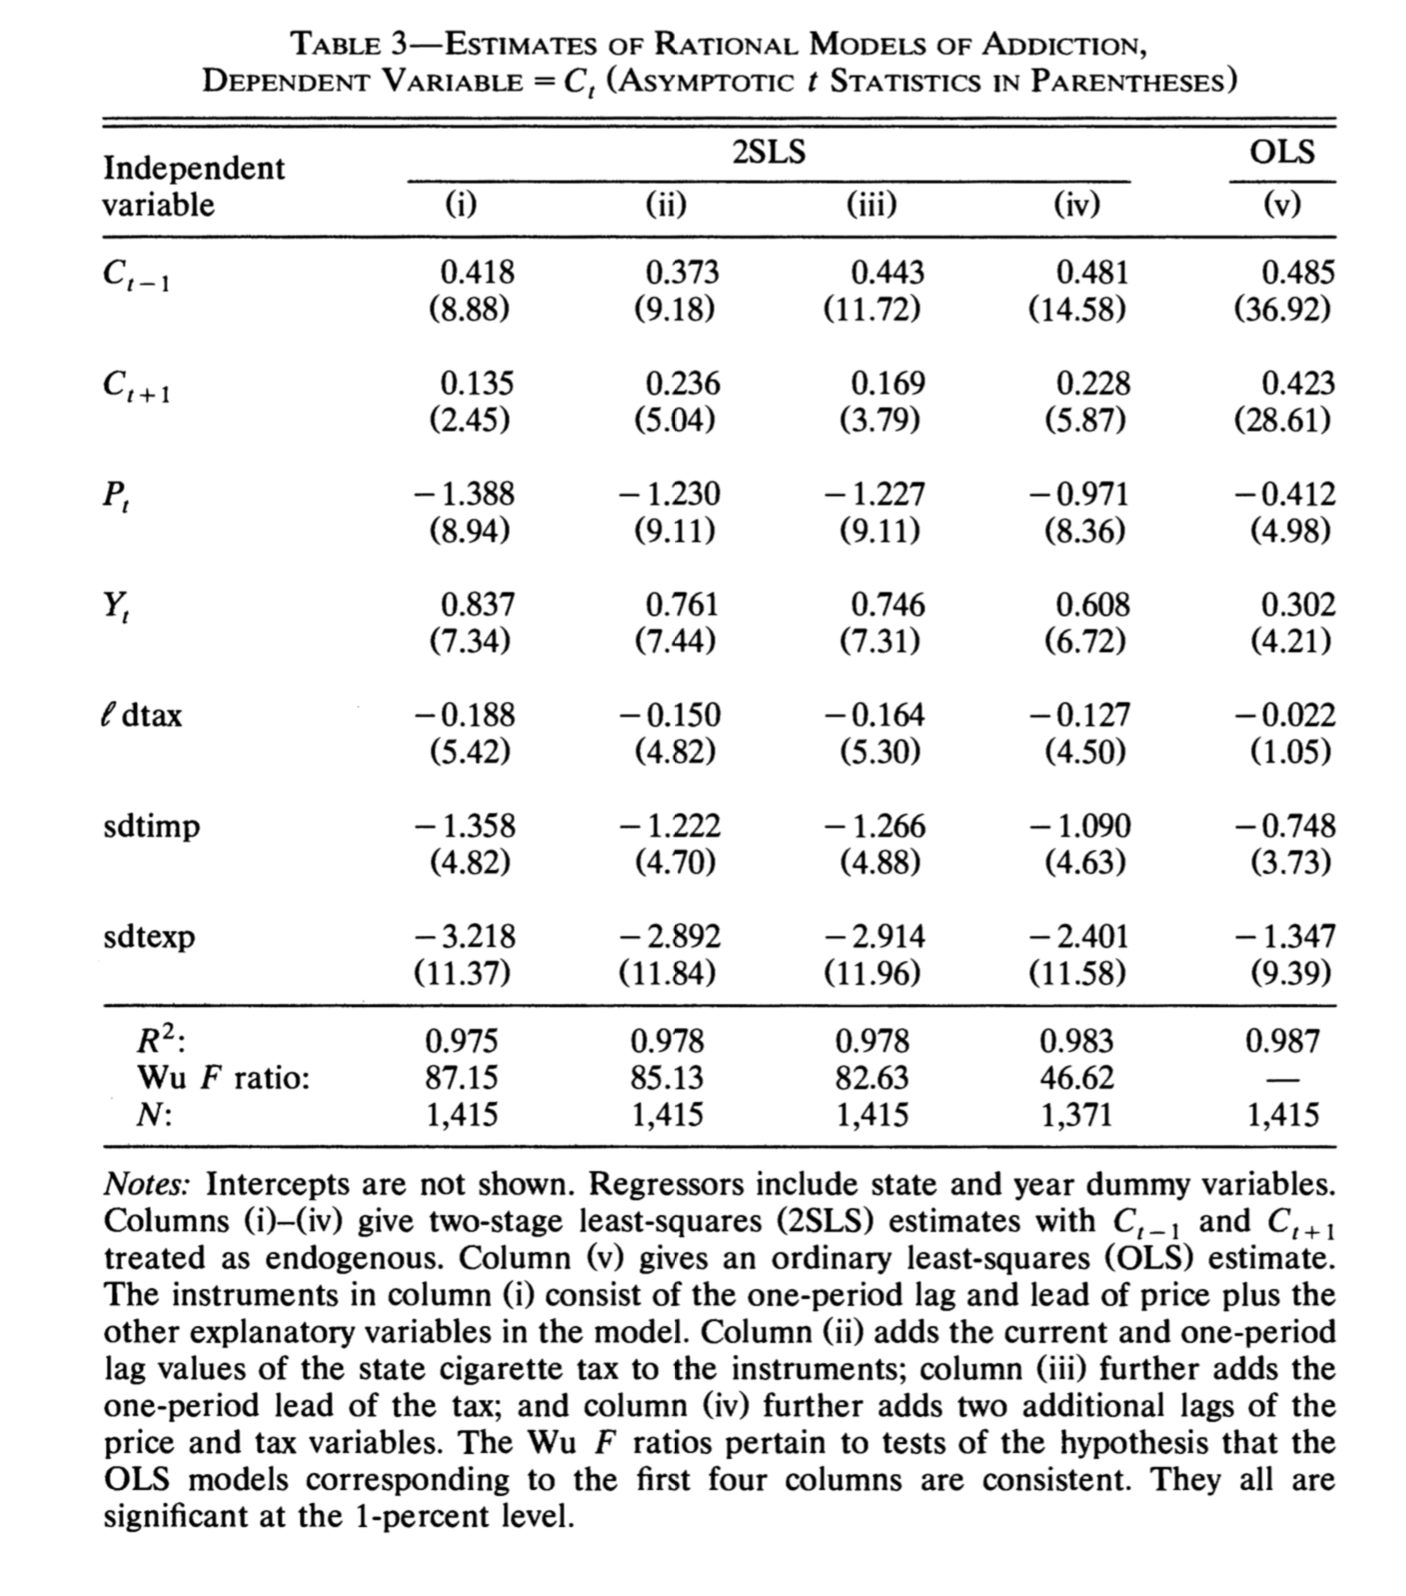
\includegraphics[width=2.8in]{./resources/gbm_t3.png}
\end{center}
\end{frame}

\begin{frame}{Becker, Grossman, Murphy (1994): Table 4}
\begin{center}
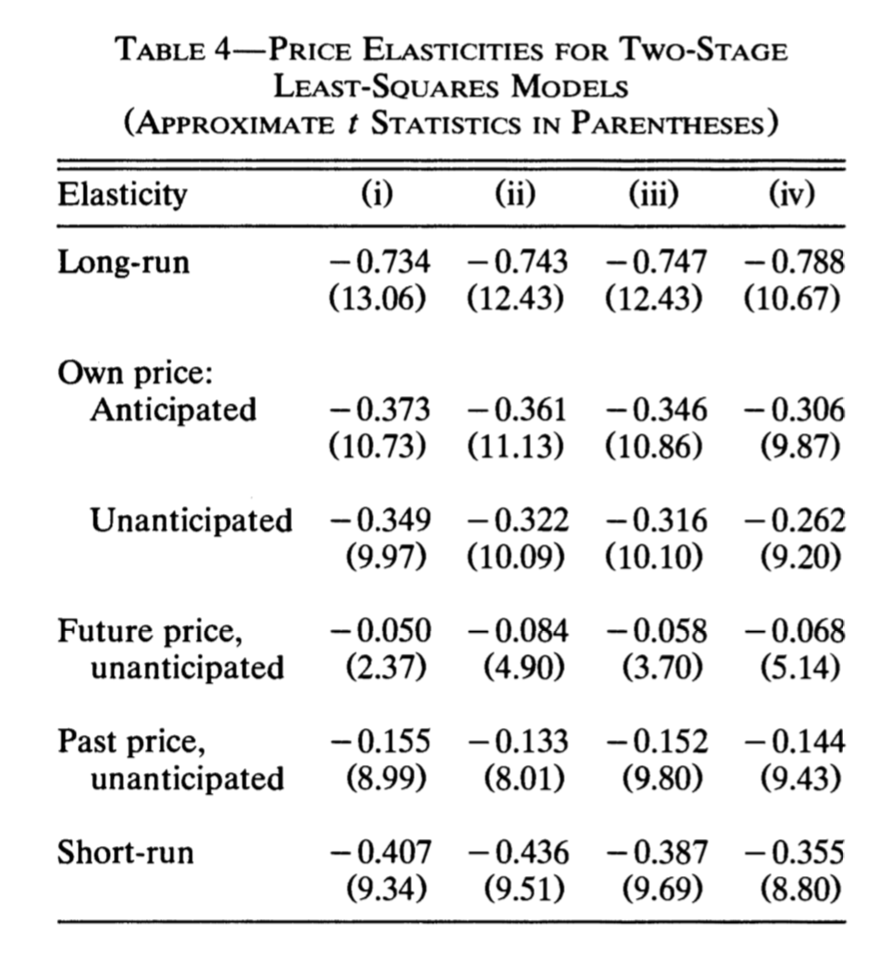
\includegraphics[width=2.5in]{./resources/gbm_t4.png}
\end{center}
\end{frame}

\begin{frame}{Becker, Grossman, Murphy (1994): Table 5}
\begin{center}
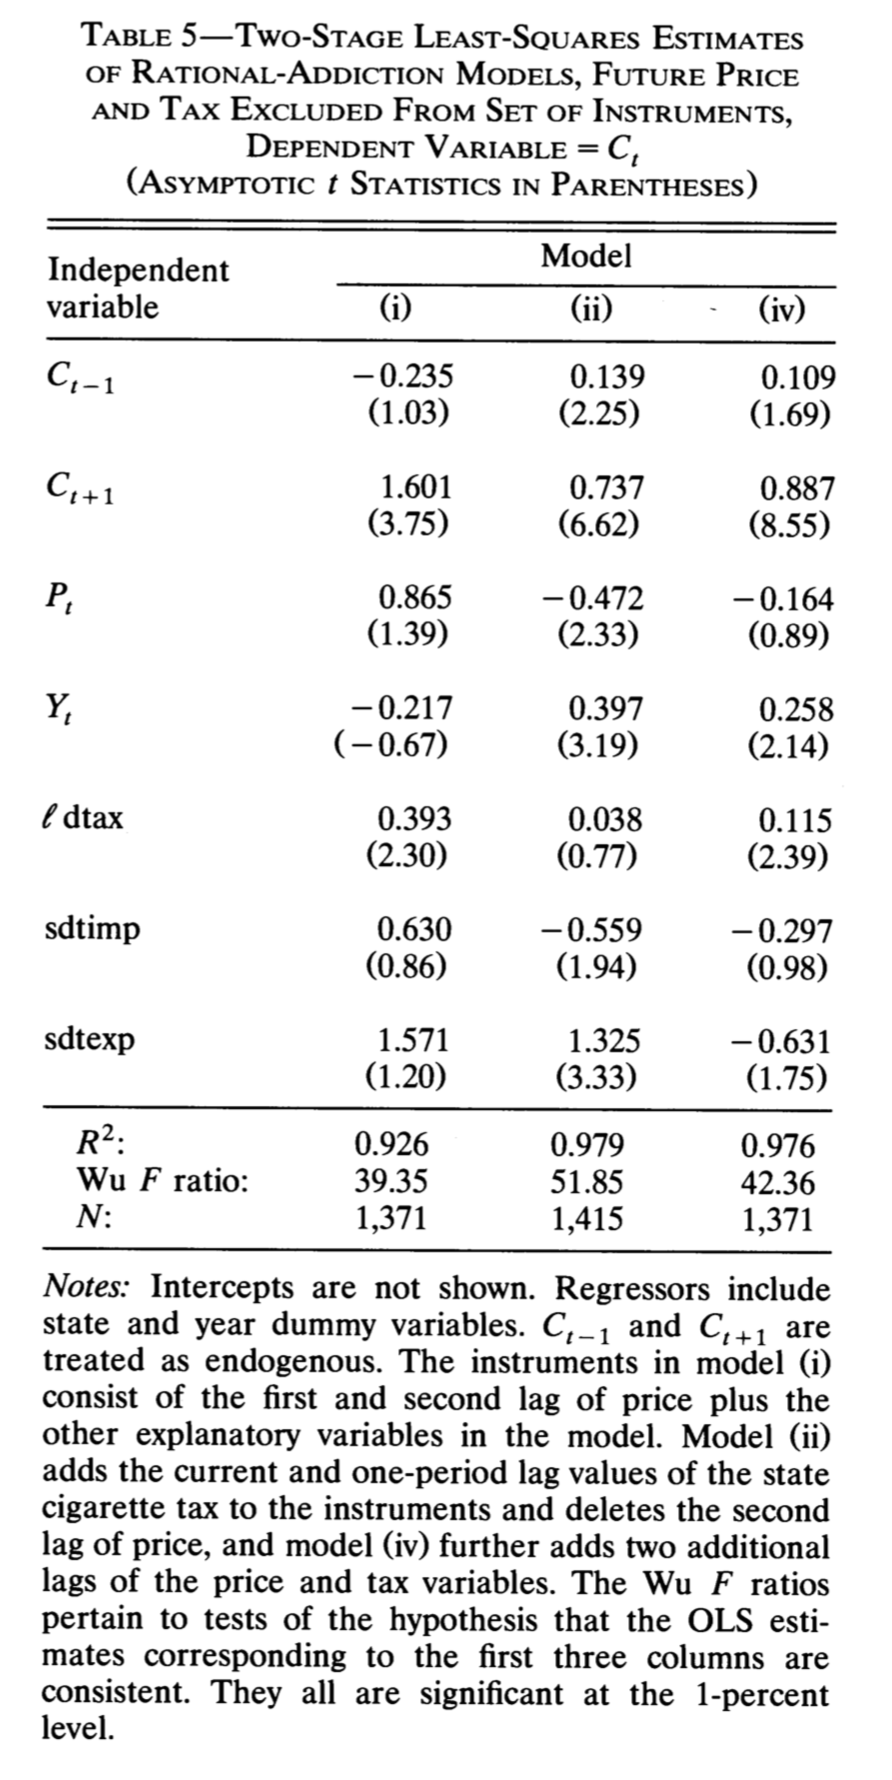
\includegraphics[width=2.3in]{./resources/gbm_t5.png}
\end{center}
\end{frame}

\begin{frame}{Becker, Grossman, Murphy (1994): Table 6}
\begin{center}
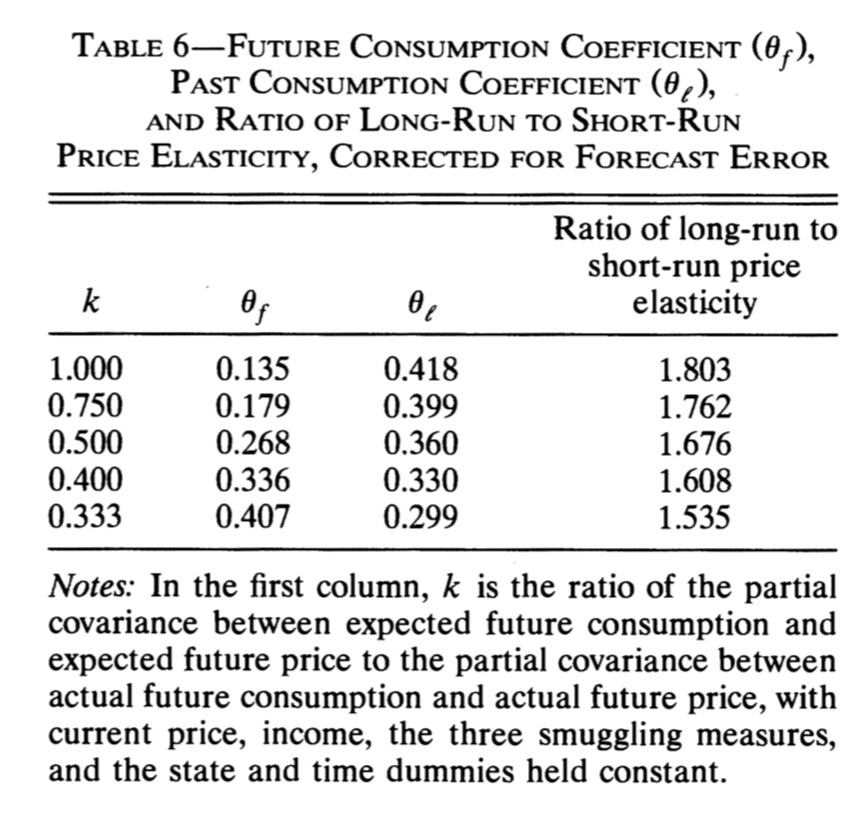
\includegraphics[width=2.3in]{./resources/gbm_t6.png}
\end{center}
\end{frame}

\begin{frame}{Becker, Grossman, Murphy (1994): Table 7}
\begin{center}
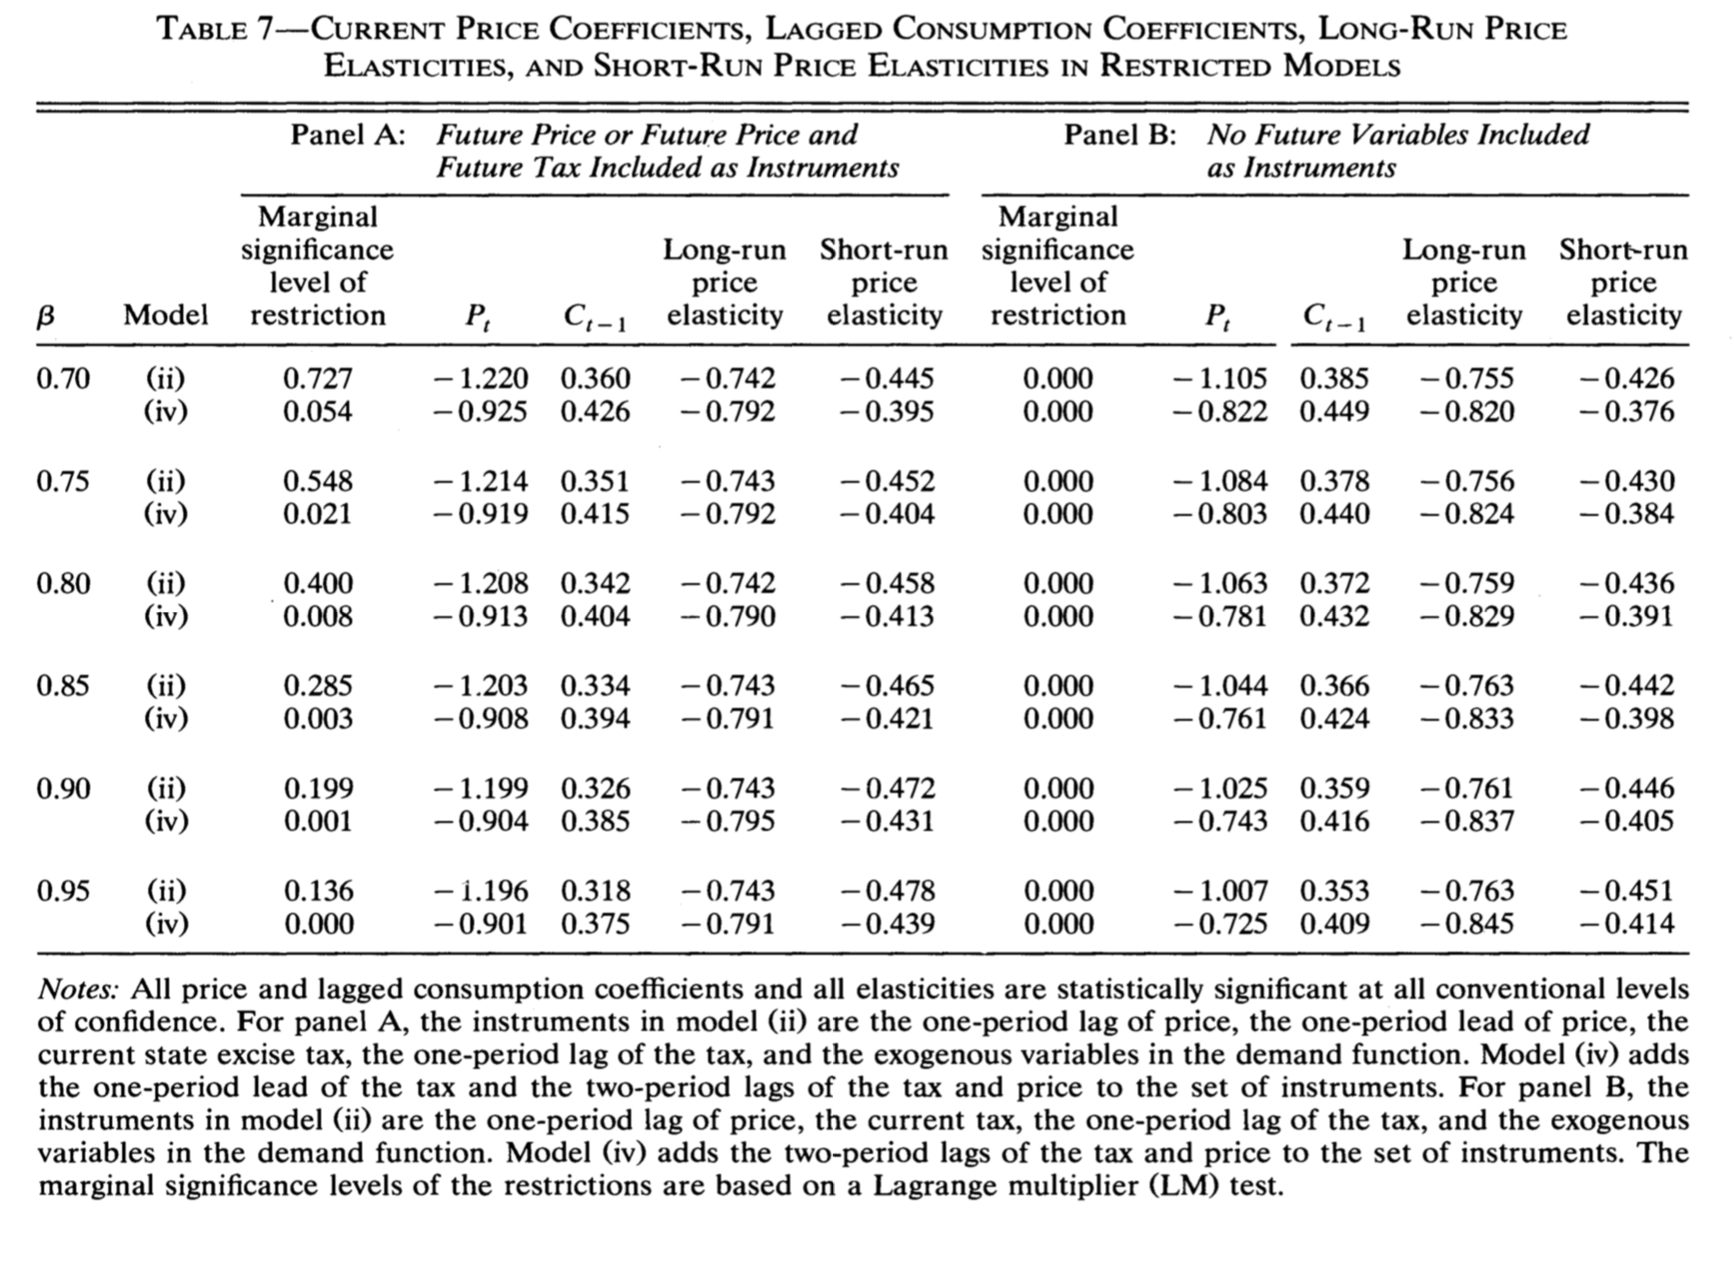
\includegraphics[width=4in]{./resources/gbm_t7.png}
\end{center}
\end{frame}


\begin{frame}{Dynamic Panel: Arellano Bond}
The main idea is that the \alert{instruments come from within the model}!
\begin{eqnarray*}
y_{it} = \rho y_{i,t-1} + x_{it}'\beta + \eta_i + \varepsilon_{it}
\end{eqnarray*}
Consider the first differences ($s$ is a dummy time index):
\begin{eqnarray*}
E\left[x_{i s}\left(\Delta y_{i t}-\rho \Delta y_{i(t-1)}-\Delta x_{i t}^{\prime} \beta\right)\right]=0
\end{eqnarray*}
Idea:
\begin{itemize}
\item Now relax \alert{strict exogeneity}.
\item Can still use $x_{is}$ as contemporaneous exogenous instrument.
\item What is an excluded instrument for $\Delta y_{i,t-1}$?
\begin{itemize}
\item Needs to be \alert{relevant}
\item Still needs to be \alert{exogenous}: not a direct determinant
\end{itemize}
%\item Estimate with GMM \texttt{pgmm} or \texttt{dynpanel}.
\end{itemize}
\end{frame}

\begin{frame}{Dynamic Panel: Arellano Bond}
\begin{eqnarray*}
E\left[x_{i s}\left(\Delta y_{i t}-\rho \Delta y_{i(t-1)}-\Delta x_{i t}^{\prime} \beta\right)\right]=0
\end{eqnarray*}
Idea: Use higher lags of $y_{it}$:
\begin{itemize}
\item $[t=2]$ or $[t=1]$: no instruments,
\item $[t=3]$:  valid instrument for $\Delta y_{i2} = (y_{i2}-y_{i1})$ is $y_{i1}$.
\item $[t=4]$:  valid instruments for $\Delta y_{i3} = (y_{i3}-y_{i2})$ is $(y_{i1}, y_{i2})$
\item$[t=5]$:  valid instruments for $\Delta y_{i4} = (y_{i4}-y_{i3})$ is $(y_{i1}, y_{i2}, y_{i3})$.
\item$[t=T]$:  valid instruments for $\Delta y_{iT-1} = (y_{i,T-1}-y_{i,T-2})$ is $(y_{i1},\ldots, y_{i,T-2})$.
\end{itemize}
Thus there are $T/(T-1)/2$ instruments
\end{frame}

\begin{frame}{Dynamic Panel: Arellano Bond}
\begin{eqnarray*}
E\left[\mathbf{y}_{i s}\left(\Delta y_{i t}-\rho \Delta y_{i(t-1)}-\Delta x_{i t}^{\prime} \beta\right)\right]=0\\
E\left[\Delta x_{it} \left(\Delta y_{i t}-\rho \Delta y_{i(t-1)}-\Delta x_{i t}^{\prime} \beta\right)\right]=0
\end{eqnarray*}
\begin{itemize}
\item $\mathbf{y}_{is}= [y_{i1},\ldots,y_{i,t-2}]$ for $t>2$.
\item \alert{Levels} instrument \alert{Differences}
\item Thus there are $T/(T-1)/2$ instruments
\item We can estimate with linear IV GMM:  \texttt{pgmm} or \texttt{dynpanel}.
\item The common complain is that \alert{instruments are still weak}.
\end{itemize}
\end{frame}

\begin{frame}{More Moments: Blundell and Bond}
\begin{align*}
E\left[\mathbf{y}_{i s}\left(\Delta y_{i t}-\rho \Delta y_{i(t-1)}-\Delta x_{i t}^{\prime} \beta\right)\right]&=0\\
E\left[\Delta y_{i,t-1} \left(y_{i t}-\rho y_{i(t-1)}- x_{i t}^{\prime} \beta\-\eta_i \right)\right]&=0\\
E\left[\Delta x_{it} \left(\Delta y_{i t}-\rho \Delta y_{i(t-1)}-\Delta x_{i t}^{\prime} \beta\right)\right]&=0
\end{align*}
\begin{itemize}
\item \alert{Differences} also instrument \alert{Levels}!
\item Important when $\rho \rightarrow 1$ or when $\sigma_u/\sigma_{\epsilon}$ becomes large.
\item These can also pin down $y_{i0}$, etc.
\item This is known as \texttt{GMM-SYS}.
\end{itemize}
\end{frame}

\begin{frame}{Recap: Dynamic Panel}
\begin{itemize}
\item Arellano Bond estimators are quite popular for a number of reasons:
\begin{itemize}
\item Easy to estimate (Linear IV)
\item Construct instruments out of the model itself.
\end{itemize}
\item Blundell Bond estimators are somewhat less popular
\begin{itemize}
\item System GMM isn't a single Linear IV problem anymore (requires full GMM).
\item Should be more efficient (more moment conditions)
\item The additional moments aren't any less reasonable that AB moments.
\end{itemize}
\item But how much do we trust using lags and levels as IV for each other?
\end{itemize}
\end{frame}


\section*{Thanks!}


\end{document}
